\newpage
%------------------------------------------------------------------
\section{Structure of the Thesis}\label{sec:intro_thesis_structure}
%------------------------------------------------------------------

This doctoral thesis is organized into six chapters.
The description and the application on a thermal-hydraulics simulation of the three statistical approaches introduced in the previous section, preceded by brief review on the selected physical models, constitute the main chapters of the present thesis (see Fig.~\ref{fig:ch1_methodological_roadmap}).
They are bookended by an introductory chapter (this chapter) and a concluding chapter.
\begin{figure}[bth]	
	\centering
	\includegraphics[width=\textwidth]{../figures/chapter1/figures/methodological_roadmap}
	\caption[The structure of thesis.]{The structure of the thesis, its main chapters.}
	\label{fig:ch1_methodological_roadmap}
\end{figure}

\textsc{Chapter~\ref{ch:trace_reflood}} gives an overview of the system thermal-hydraulics code \gls[hyper=false]{trace} with an emphasis on its reflood phenomena modeling and simulation.
The chapter also introduces the reflood experiment at the \gls[hyper=false]{feba} facility which serves as the experimental basis of this work.
The chapter includes the selection of initial parameters relevant for reflood simulation and the propagation of their uncertainties on the code prediction.

\textsc{Chapter~\ref{ch:gsa}} provides the application of statistical sensitivity analysis method for the reflood model.

\textsc{Chapter~\ref{ch:gp_metamodel}}

\textsc{Chapter~\ref{ch:bayesian_calibration}}

\textsc{Chapter~\ref{ch:conclusions}}

%\begin{sidewaysfigure}
%	\centering
%	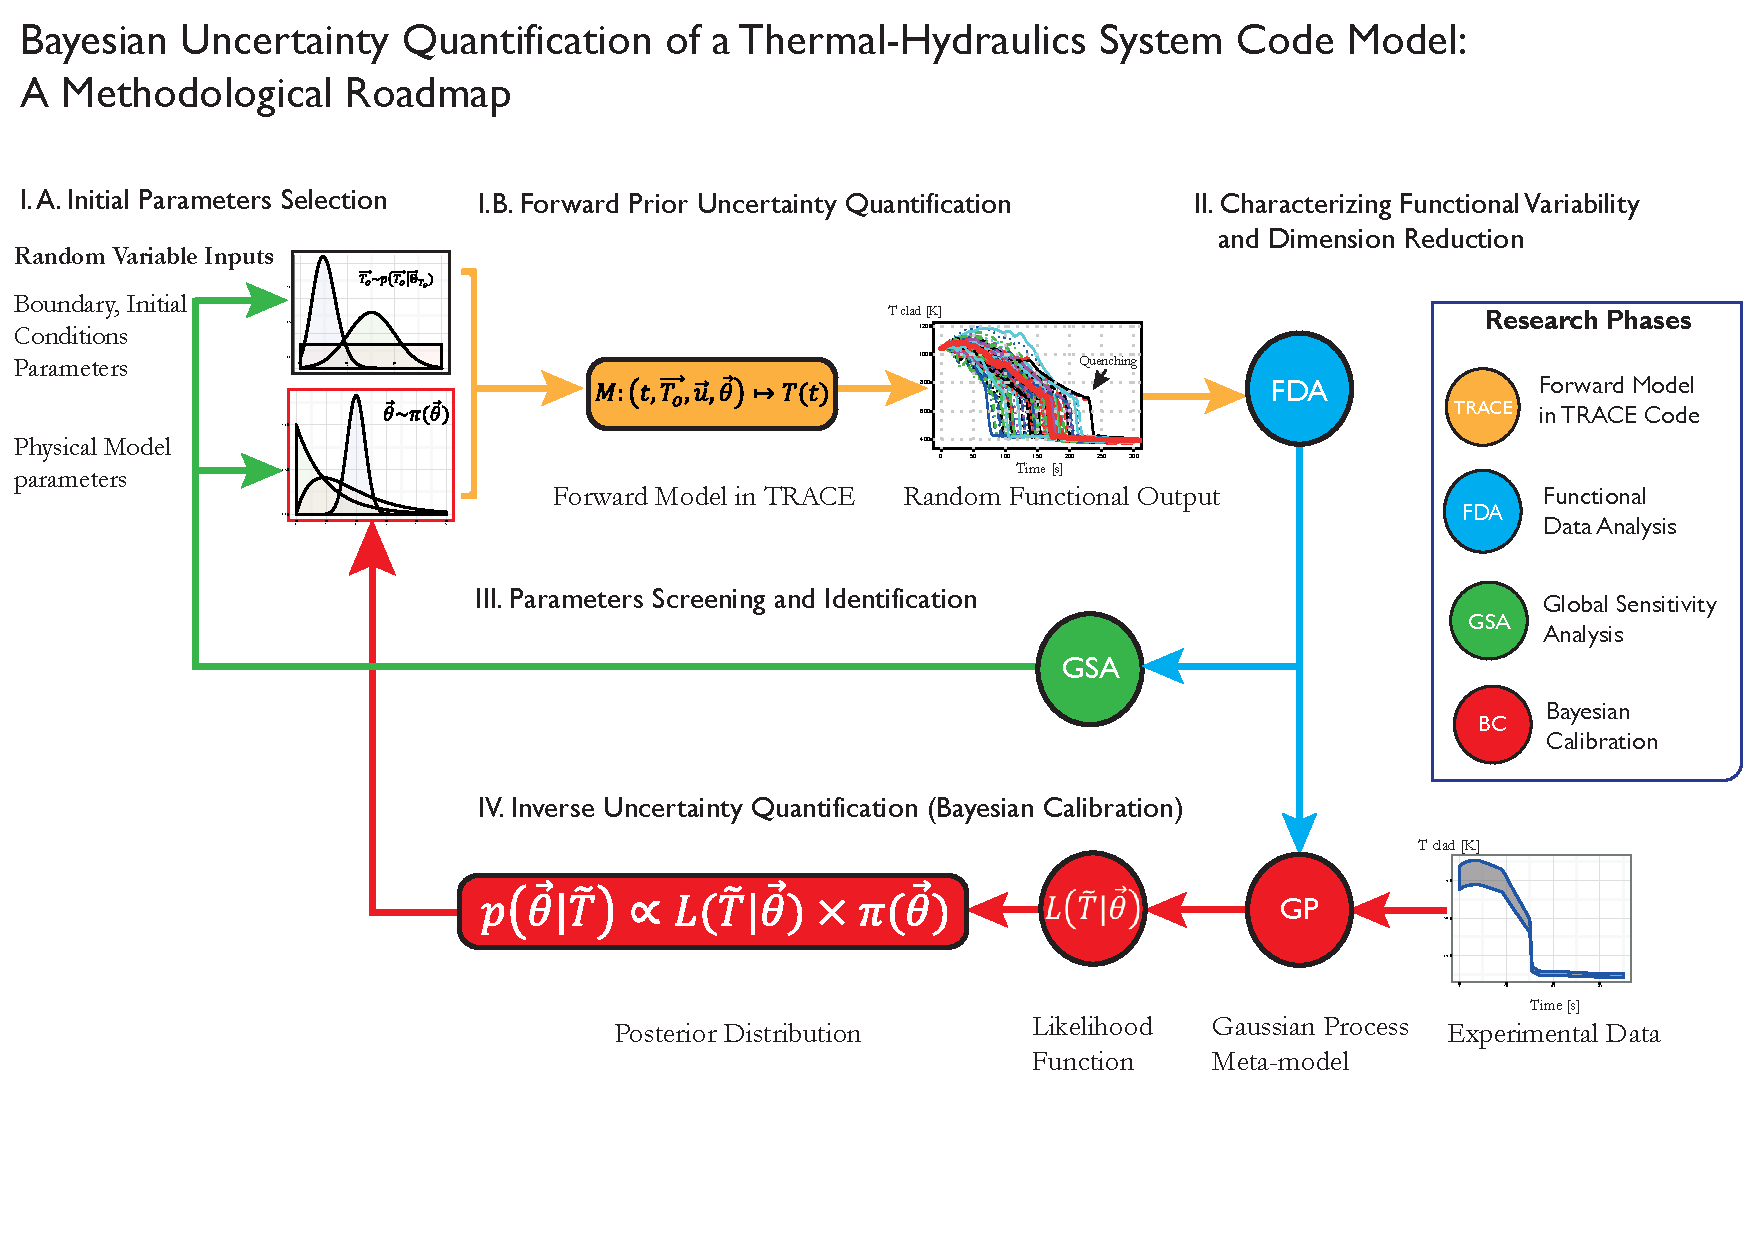
\includegraphics[width=0.85\textwidth]{../figures/methodologicalRoadmap/methodologicalRoadmap.pdf}
%	\caption{Methodological Roadmap of the Thesis}
%	\label{fig:methodological_roadmap}
%\end{sidewaysfigure}